%! TEX program = xelatex
\documentclass[12pt,a4paper]{article} 

\usepackage[T1]{fontenc}
\usepackage[utf8]{inputenc} 
\usepackage{amsmath, graphicx, enumerate}
\usepackage[polish]{babel}
\usepackage{minted}
\usepackage{url}
\usepackage{dirtree}


\graphicspath{ {images} }

\usepackage{biblatex} %Imports biblatex package
\addbibresource{references.bib} %Import the bibliography file

\pagenumbering{gobble}
\begin{document}
\title{{
  % \begin{center}
  %   \includegraphics[width=8cm]{school-logo}
  % \end{center}
  \vspace{1.3cm}
  \LARGE Technologie IoT - Programowanie Python \\
  \LARGE Klon gry Asteroids}}
\author{{\Large My Name, w12345}}
\date{}
\maketitle
\newpage


\section{Opis projektu}
  Celem projektu jest wykonanie gry zainspirowanej grą Asteroids \cite{asteroids} w bibliotece Pygame \cite{pygame}. Motywem gry jest tester kontrolerów, włączając grę widzimy narysowany kontroller do gier na wzór kontrolera do konsoli NES.

  \begin{figure}[h!]
  \begin{center}
    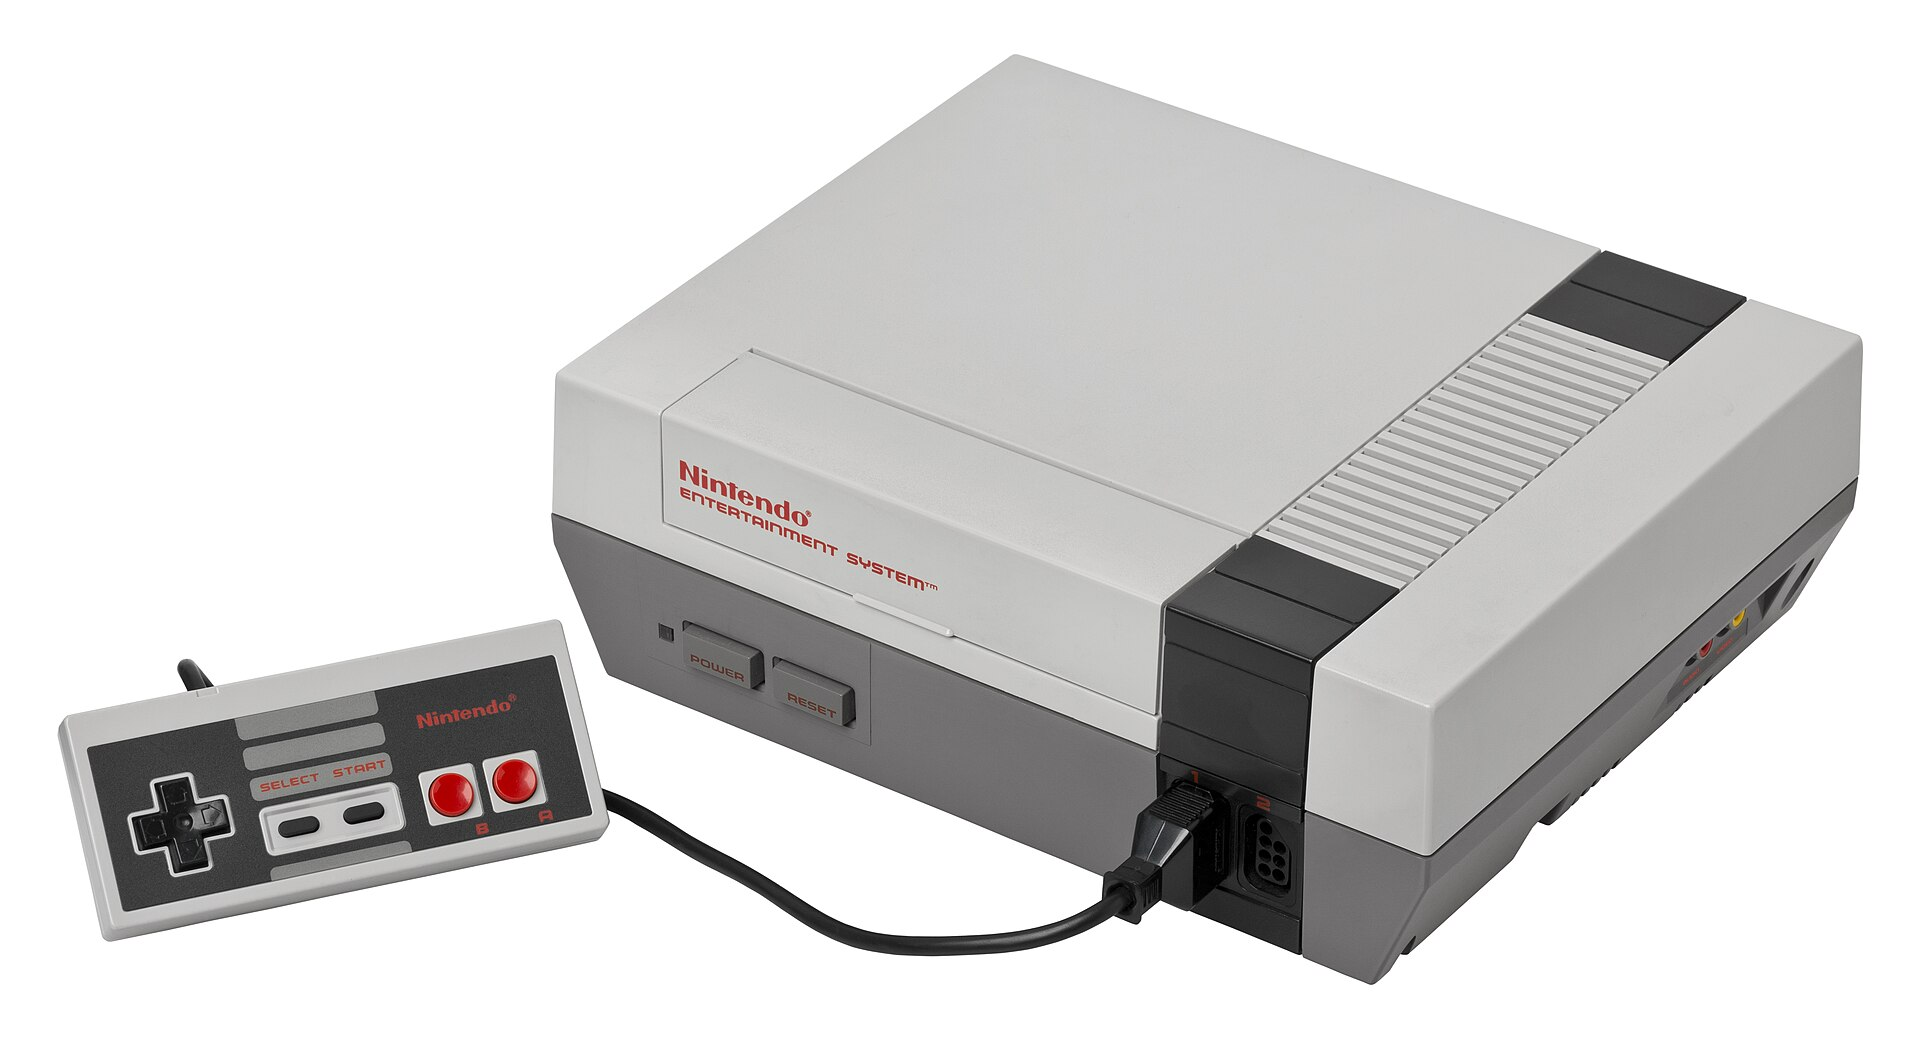
\includegraphics[width=8cm]{images/NES-Console-Set.jpg}
  \end{center}
  \caption{Nintendo Entertainment System}
  \label{fig:nes}
  \end{figure}

\noindent Wszystkie przyciski widoczne w menu gry podswietlają się w momencie wcisnięcia ich na kontrolerze, brakuje tu gałek analogowych i triggerów z typowych kontrolerów, jednak kontroler konsoli NES ich nie posiadał.

    \begin{figure}[h!]
  \begin{center}
    \includegraphics[width=\textwidth]{images/ekran-tytułowy.png}
  \end{center}
  \caption{Menu gry}
  \label{fig:nes}
  \end{figure}
  
\newpage
\noindent Rozgrywka rozpoczyna się po wcisnięciu przycisku START, zostaje wtedy wykonana animacja oddalająca kontroler, pojawiają się napisy informujące o punktach oraz życiu gracza, asteroidy zaczynają się pojawiać, a nam zostaje dana możliwość kontroli naszego 'statku'.

  \begin{figure}[h!]
  \begin{center}
    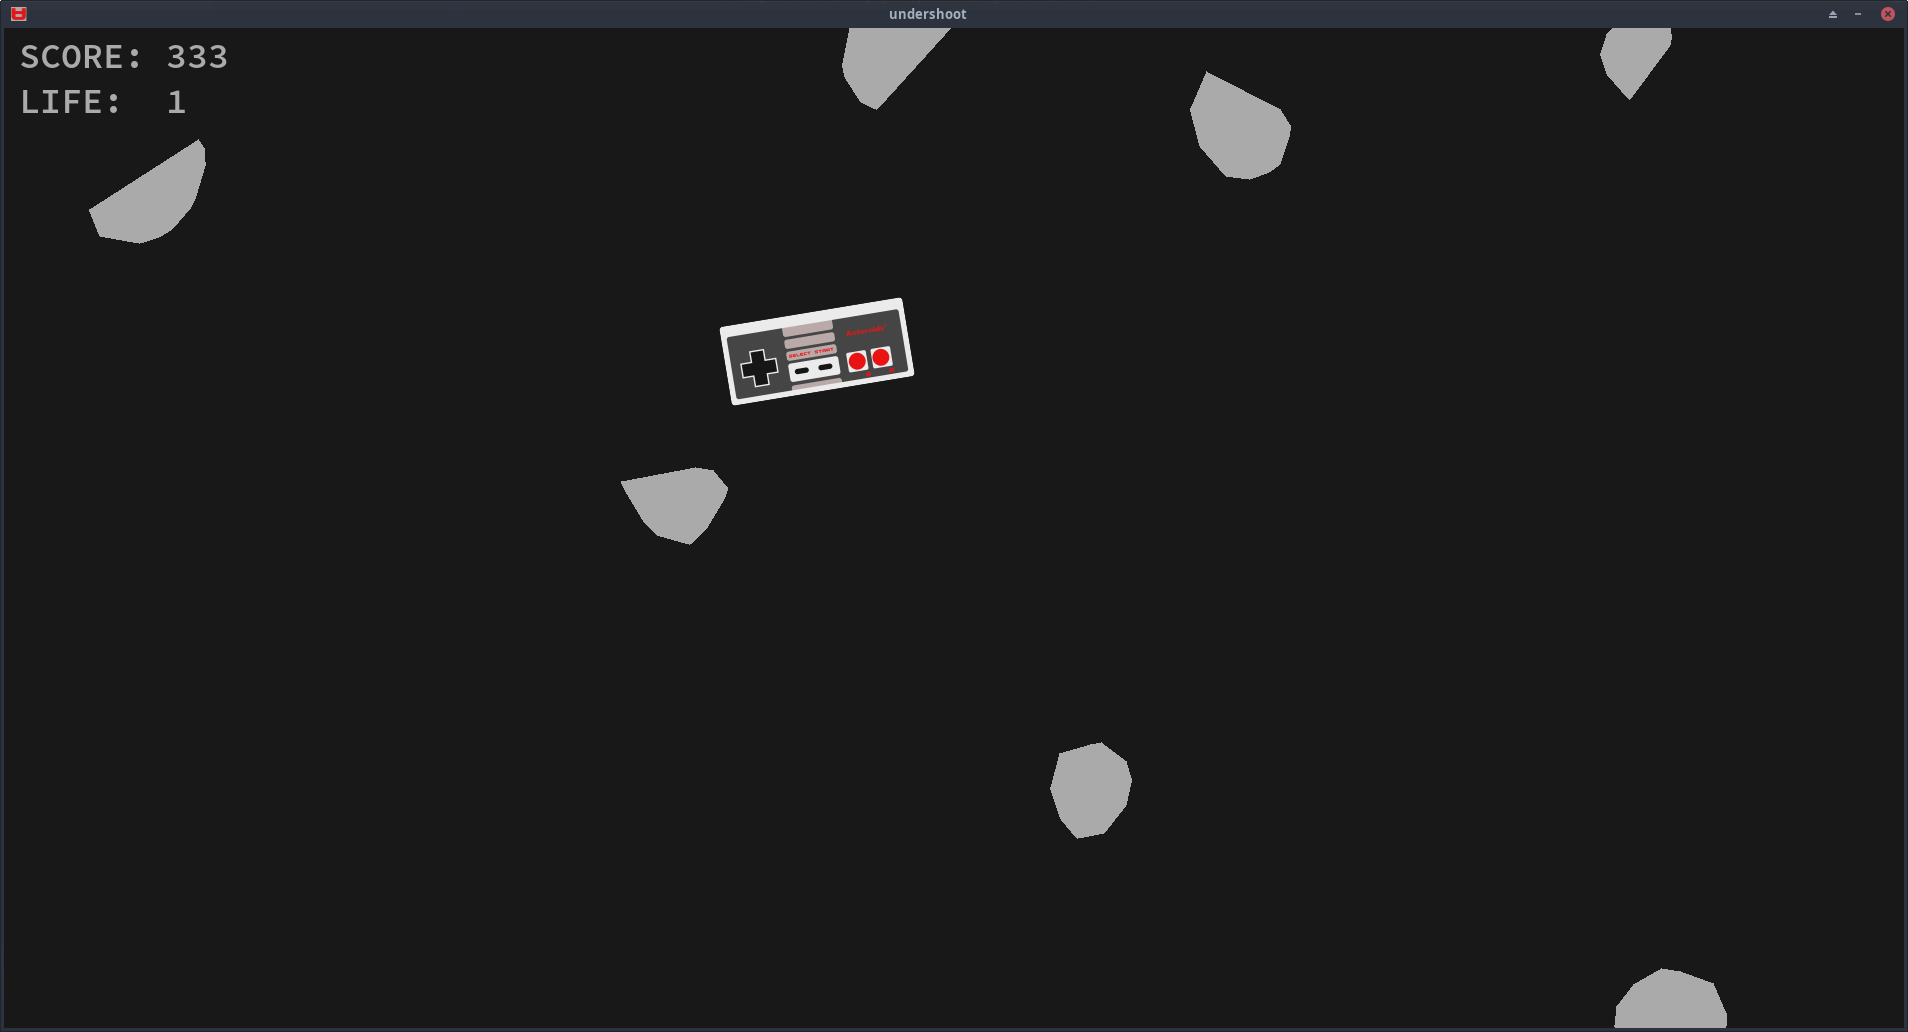
\includegraphics[width=\textwidth]{images/przyklad-gry.png}
  \end{center}
  \caption{Rozgrywka}
  \label{fig:nes}
  \end{figure}

\noindent Naszym zadaniem jest strzelanie do i unikanie asteroid, jeżeli asteroida uderzy w nas 3 razy, pokazuje się ekran informujący o przegranej oraz o zdobytej liczbie punktów.

  \begin{figure}[H]
  \begin{center}
    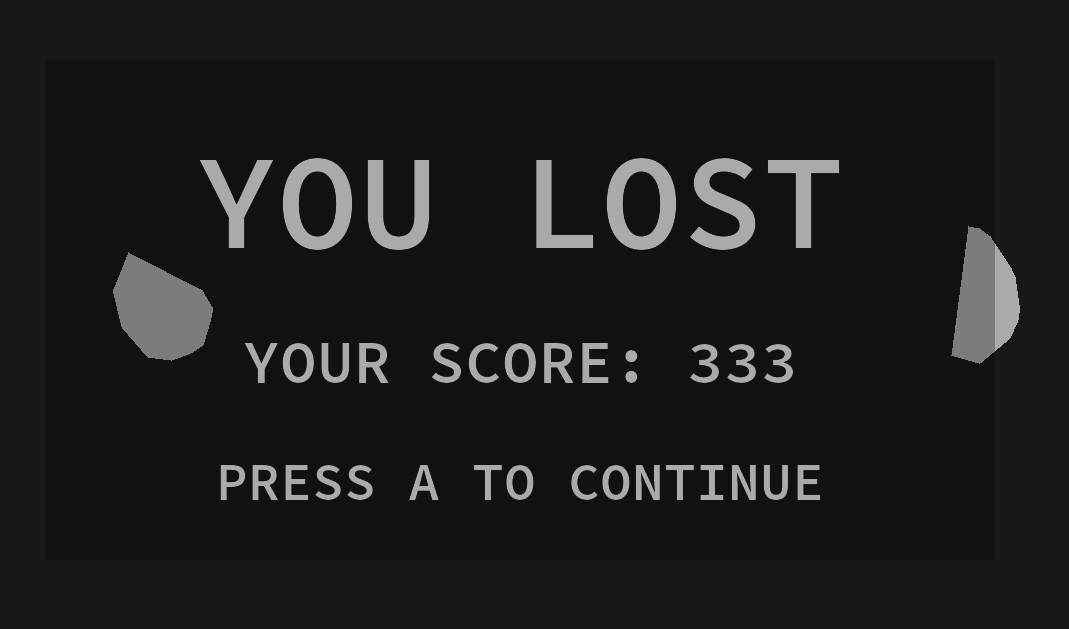
\includegraphics[width=10cm]{images/przegrana2.png}
  \end{center}
  \caption{Przegrana}
  \label{fig:nes}
  \end{figure}

  \newpage

\section{Struktura projektu}
\subsection{Lista plików}

\dirtree{%
.1 Projekt.
.2 conf.py .
.2 dpad.py .
.2 entity.py .
.2 lost\_screen.py .
.2 misc.py .
.2 polygon.py .
.2 separation\_axis\_theorem.py.
.2 tester.py .
.2 undershoot .
.2 fonts/ .
.3 Need Every Sound.ttf .
.3 NintendBoldRM8E.ttf .
.3 SourceCodePro.ttf .
.2 images/ .
.3 icon.png .
}

\vspace{\baselineskip}
\noindent Plik \textbf{undershoot} (plik .py) jest plikiem głównym, w nim znajduje się główna pętla gry oraz inicjalizacja wszystkich systemów i importowanie reszty plików.
\vspace{\baselineskip}

\noindent Plik \textbf{conf.py} zawiera większość zmiennych konfiguracyjnych, dużo plików importuje jego zawartość.

\vspace{\baselineskip}
\noindent Pliki \textbf{tester.py} oraz \textbf{dpad.py} są odpowiedzialne za tworzenie powierzchni (surface) z narysowanym kontrolerem, \textbf{lost\_screen.py} zawiera funkcję tworzącą powierzchnię widoczną po przegraniu.

\vspace{\baselineskip}
\noindent \textbf{enitity.py} i \textbf{polygon.py} to obiekty gry, \textbf{separation\_axis\_theorem.py} jest importowane przez \textbf{polygon.py} i jest zewnętrzną biblioteką używaną do sprawdzenia kolizji między dwoma wielokątami.

\vspace{\baselineskip}
\noindent Reszta plików to czcionki oraz ikona gry.
  \newpage

  \subsection{Inicjalizacja i pętla gry}
  Uproszczona struktura programu wygląda w następujący sposób:
  
\begin{minted}{python}
# import and initialize everything...
player = Player()
asteroids, projectiles = [], []

delta_time = get_dt()
running = True
while running:
    buttons = handle_input_events()

    maybe_spawn_asteroid(asteroids, delta_time)

    player.update(buttons, delta_time)
    for asteroid in asteroids:
        asteroid.update(delta_time)
        if asteroid.collides(player):
            # handle collision
            player.kill_or_something()
    for projectile in projectiles:
        projectile.update(delta_time)
        # ...

    screen.clear()
    for entity in entity_list:
        entity.draw()
    screen.flip()
    
    delta_time = get_dt()
\end{minted}

\noindent Nie została tu pokazana pętla menu głownego. Dodatkowo, w rzeczywistości program jest dużo bardziej rozbudowany. 
Wiele logiki, takiej jak sprawdzanie kolizji i wykonanie jej skutków, znajduje się w pierwszej warstwie pętli (zamiast być głebiej ukryte, za kilkoma wywołaniami funkcji). W przypadku tak prostej i krótkiej gry, taka struktura dużo upraszcza.

\newpage
\subsection{Abstrakcje}
Główne abstrakcje wykorzystywane w programie to:
\begin{itemize}
\item klasa \texttt{Entity} i klasy dziedziczące,
\item klasa \texttt{Polygon},
\item funkcja \texttt{make\_controller\_surface()}
\end{itemize}

\vspace{\baselineskip}
\noindent Entity zawiera właściwości fizyczne, tj. pozycję, orientację, ruch oraz przyśpieszenie.
Każde Entity musi posiadać hitbox - obiekt klasy Polygon wykorzystywany w metodzie Entity.collides().
Dodatkowo, każde Entity może implementować metody .update() oraz .draw().
Z Entity dziedziczą klasy Player, Asteroid i Projectile.

\vspace{\baselineskip}
\noindent Polygon jest wykorzystywany jedynie jako hitbox należący do klasy Entity.

\vspace{\baselineskip}
\noindent Player, klasa dziedzicząca z Entity, wykorzystuje make\_controller\_surface() przy użyciu metody .draw().
Zwrócona powierzchnia kontrolera z narysowanymi aktualnie wciśniętymi przyciskami jest transformowana(rotacja, skalowanie) i rysowana w pozycji pozycji obiektu Player.


\section{Działanie różnych systemów}
% @todo: https://en.wikipedia.org/wiki/Delta_timing?useskin=vector
\subsection{Delta time}
Delta time \cite{dt} to czas od ostatniej iteracji pętli, przekazywanie jej do funkcji zmieniającej stan gry jest konieczne, aby zachować tą samą prędkość fizyki gry, przy różnych ilościach klatek na sekundę.

\subsection{Symulacja fizyki}
Poruszanie się obiektów w grze jest wykonane w bardzo prosty sposób, każdy obiekt posiada wektory pozycji, przyśpieszenia oraz
ruchu. Przy każdym użyciu metody .update() następuje:
\begin{minted}{python}
def update(self):
    self.velocity += self.acceleration
    self.position += self.velocity
\end{minted}
Takie operacje są lepiej opisane w książce The Nature of Code, dział 1.10 'Interactivity with Acceleration' \cite{noc}.
% @todo: https://natureofcode.com/book/chapter-1-vectors/

\vspace{\baselineskip}
\noindent Następnie występuje rotacja obiektów o 'rotation\_velocity', w tym wypadku hitbox obiektu musi zostać obrócony.
Metoda .rotate() w klasie Polygon:
\begin{minted}{python}
def rotate(self, angle):
    self.points = [ (p - self.middle).rotate(angle) + self.middle 
                                             for p in self.points ]
\end{minted}
środek (middle) to punkt równy średniej wszystkich innych punktów wielokąta.

\vspace{\baselineskip}
\noindent Kolizje między obiektami są sprawdzane przy pomocy dwóch funkcji, na początku zostaje wywołane maybe\_collides():
\begin{minted}{python}
def maybe_collides(self, polygon):
    x1, x2, y1, y2 = self.rect_coords
    for x, y in polygon.rect_points:
        if x1 <= x <= x2 and y1 <= y <= y2:
            return True
    return False
\end{minted}

\noindent rect\_coords to współrzędne a rect\_points to punkty prostokąta, który jest wrysowany sprawdzany wielokąt.
Są one aktualizowane przy użyciu metod .move() oraz .rotate().
Użycie tej metody jest bardzo szybkie, dlatego dopiero w sytuacji kiedy maybe\_collides() zwraca True, używana jest metoda collides().

\vspace{\baselineskip}
\noindent collides() korzysta z algorytmu Separating Axis Theorem \cite{collisions} \cite{SAT}, do którego została użyta zewnętrza biblioteka \cite{SATlib} % @todo

\subsection{Generacja asteroid}
Generacja asteroid jest niekompletna - nie możemy ustawić rozmiaru asteroidy i generowane są niedokładne, mają zbyt małą lub zbyt dużą ilość kątów.
\begin{minted}{python}
points = [ Vector2(position) ]
start = Vector2(1, 0)

for _ in range(9):
    start = start.normalize() * random.randint(400, 2000) / 50
    start = start.rotate(random.randint(80, 600)/10)
    points.append(points[-1] + start)
\end{minted}
możliwymi zmianami algorytmu jest liczenie długości boków, sumy kątów, zmiana zakresu liczb użytego w funkcjach losowych (prawdopodobnie w zależności od chcianego rozmiaru), sprawdzanie pozycji pierwszego punktu wobec pierwszego punktu.


\subsection{Tworzenie nowych asteroid}
Nowe asteroidy pojawiają się na mapie losowo, z szansą wynoszącą 10 + 5k na jedną minutę, gdzie k=liczba minut.
\begin{minted}{python}
rate = 10 + 5*minutes
chance = int(rate * delta_time*100) 
if random.randint(0, 60*1000*100) < chance:
    asteroids.append(Asteroid(player=p))
\end{minted}
mnożenie delta\_time (liczba ms) przez 100 służy dokładności, mnożenie przez 1000 jest konieczne, ponieważ ten kod wykonuje się wiele razy w ciągu jednej sekundy.

\printbibliography %Prints bibliography

\end{document}
